%! suppress = MissingImport
\begin{wrapfigure}{r}{0.3\textwidth}
    \centering
    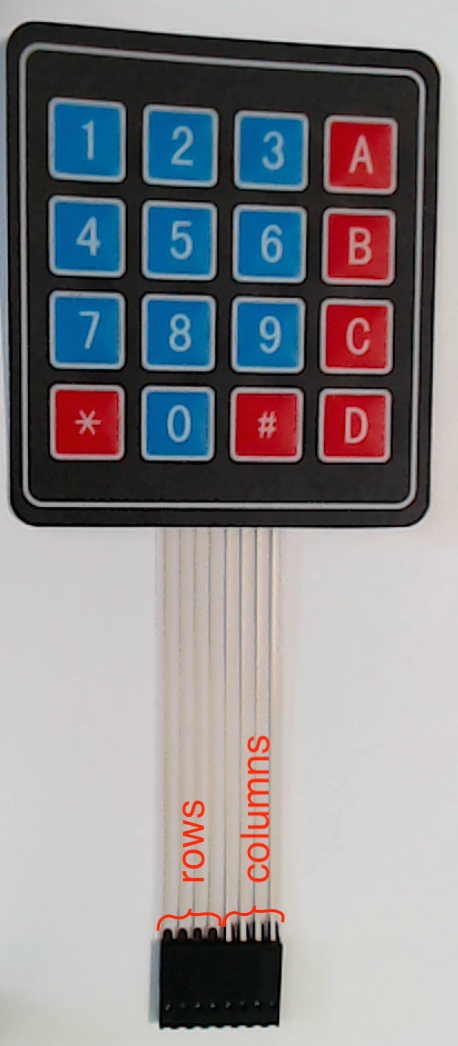
\includegraphics[width=0.25\textwidth]{keypad/keypad-annotated}
    \caption{The numeric keypad's header has four row pins and four column pins. \label{fig:keypad-annotated}}
\end{wrapfigure}

Observe that the matrix keypad has sixteen buttons has eight pins in its female connector.
As shown in Figure~\ref{fig:keypad-annotated}, when the keypad is face-up and oriented for reading, the four pins on the left are the \textit{row} pins, and the four pins on the right are the \textit{column} pins.
From left-to-right, we will name these pins \texttt{row1}, \texttt{row4}, \texttt{row7}, \texttt{row*}, \texttt{column1}, \texttt{column2}, \texttt{column3}, \texttt{columnA}.

Figure~\ref{fig:keypad-diagram} shows a diagram of the wiring for the matrix keypad.

\begin{figure}[p]
    \centering
    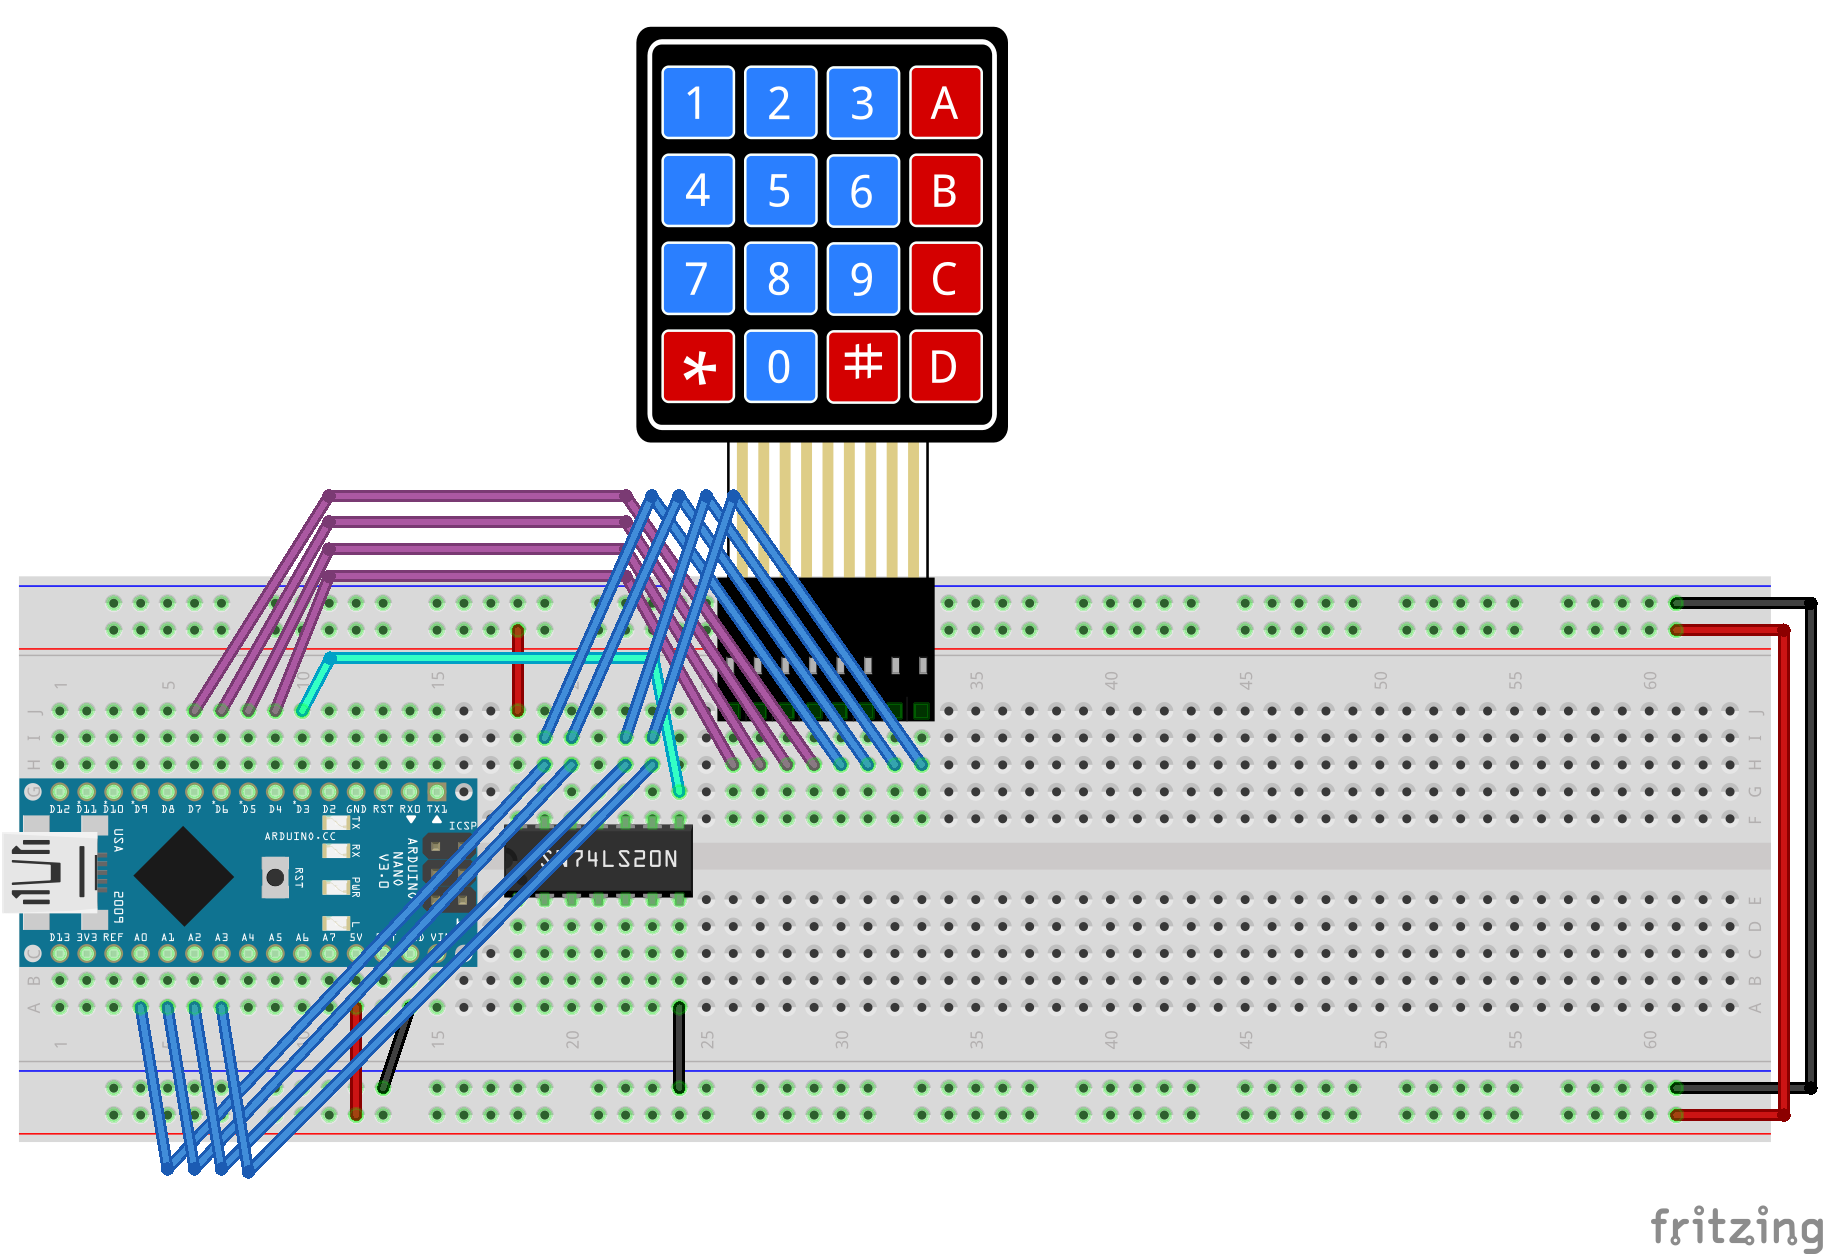
\includegraphics[width=0.9\textwidth]{fritzing_diagrams/keypad}
    \caption{Diagram of wiring associated with matrix keyboard input.
        \textit{Note: connection between the 74LS20's pin 8 and the \developmentboard's
        \texttt{D3} pin was previously installed in Section~\ref{subsec:nand}.}
        \label{fig:keypad-diagram}}
\end{figure}

If your 8-pin male-male header strip is not already inserted into the keypad's female connectors, insert it into the female connectors now.
If your male-male header strip has more than eight pins, position the excess pins to the right of the column pins.
Connect your keypad to your breadboard such that \texttt{row1} is in contact point j26, and \texttt{columnA} is in contact point j33 (and any unused pins on the male-male header are in contact points j34, j35, etc.);
see Figure~\ref{fig:keypad-header}.

Peel off a 4-conductor cable from the \rainbow.
Insert one end in contact points h26-h29, in the same breadboard rows as the keypad's row pins (Figure~\ref{fig:keypad-row-cable}).
Insert the other end of the cable in contact points j9-j6 (Figure~\ref{fig:keypad-row-nano}).
You want the \developmentboard's \texttt{D4} pin to connect to the keypad's \texttt{row1} pin, \texttt{D5} to \texttt{row4}, \texttt{D6} to \texttt{row7}, and \texttt{D7} to \texttt{row*} (Figure~\ref{fig:keypad-row-full}).

Peel off another 4-conductor cable from the \rainbow.
Insert one end in contact points h30-h33, in the same breadboard rows as the keypad's column pins.
Insert the other end of the cable in contact points i19, i20, i22, and i23 (electrically connected to the 74LS20's \texttt{D2}, \texttt{C2}, \texttt{B2}, and \texttt{A2}: pins 13, 12, 10, and 9).
See Figure~\ref{fig:keypad-col-nand}.
Peel off another 4-conductor cable from the \rainbow.
Insert one end in contact points h19, h20, h22, and h23.
Insert the other end in contact points a4-a7 (electrically connected to the \developmentboard's \texttt{A0}-\texttt{A3} pins).
See Figure~\ref{fig:keypad-col-nano}.

\begin{figure}
    \centering
    \subfloat[The matrix keypad's connector, with the male-male header strip, just before being inserted into the breadboard.
        Note the excess header strip's excess pin to the right of the column pins, in contact point j34.]{
        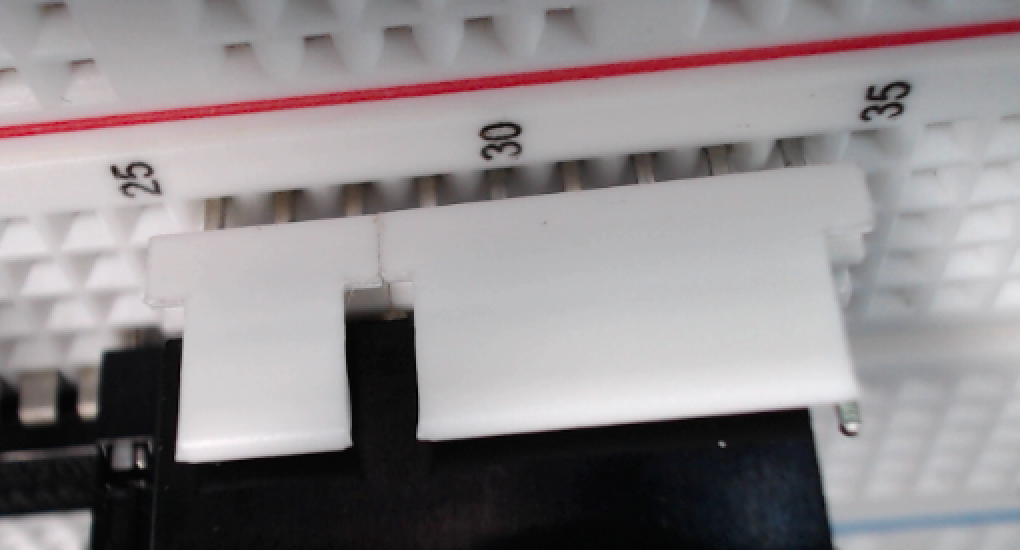
\includegraphics[width=.5\textwidth]{keypad/keypad-header}
        \label{fig:keypad-header}
    }
    \hfil
    \subfloat[One end of the ``rows'' cable electrically connected to the keypad's row pins.]{
        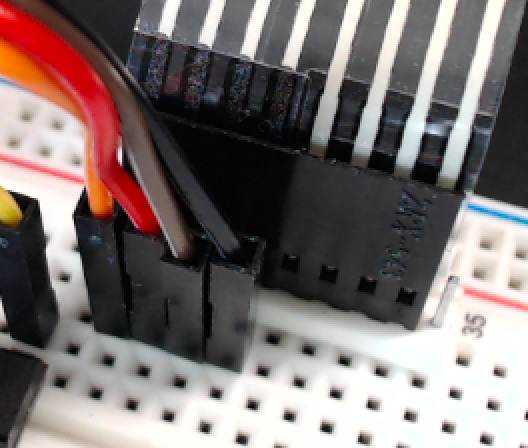
\includegraphics[width=.4\textwidth]{keypad/keypad-row-cable}
        \label{fig:keypad-row-cable}
    }

    \subfloat[The other end of the ``rows'' cable electrically connected to the \developmentboard's \texttt{D4}-\texttt{D7} pins.]{
        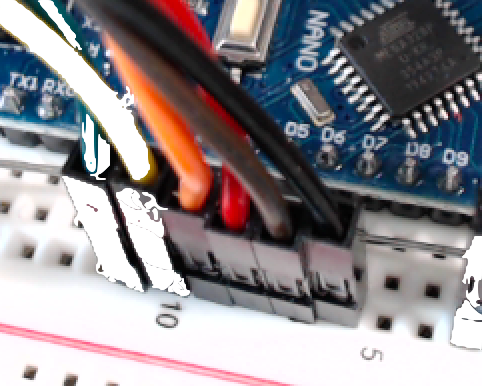
\includegraphics[width=.4\textwidth]{keypad/keypad-row-nano}
        \label{fig:keypad-row-nano}
    }
    \hfil
    \subfloat[Connection between the keypad's row pins and the \developmentboard's
        \texttt{D4}-\texttt{D7} pins.]{
        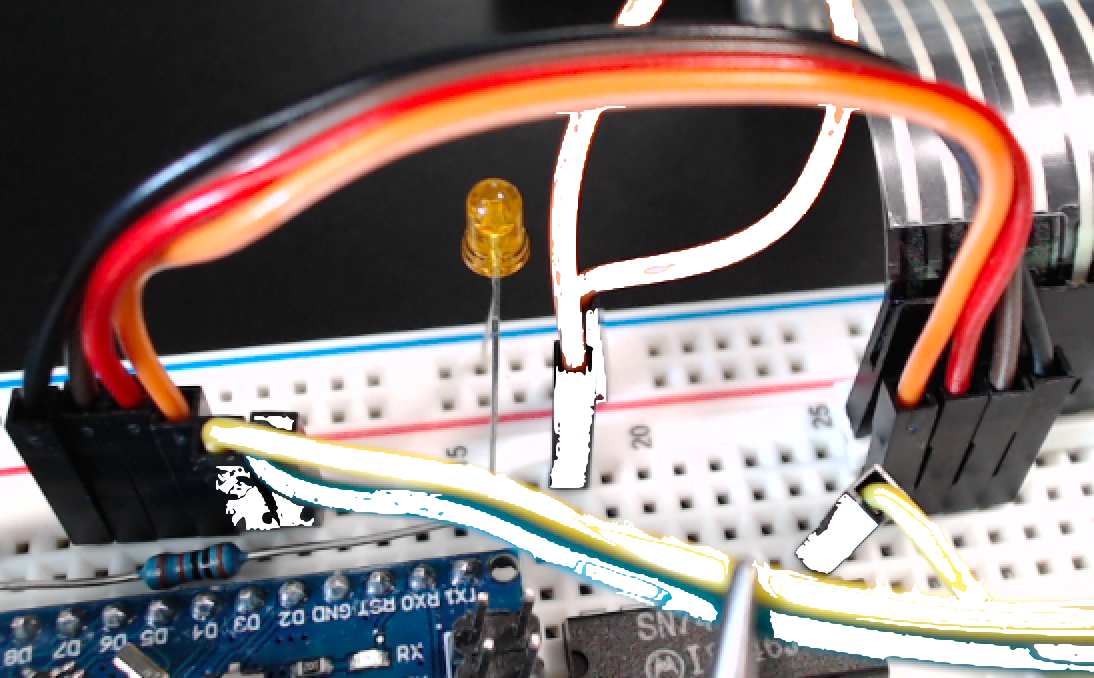
\includegraphics[width=.5\textwidth]{keypad/keypad-row-full}
        \label{fig:keypad-row-full}
    }

    \subfloat[Connection between the keypad's column pins and the 74LS20.]{
        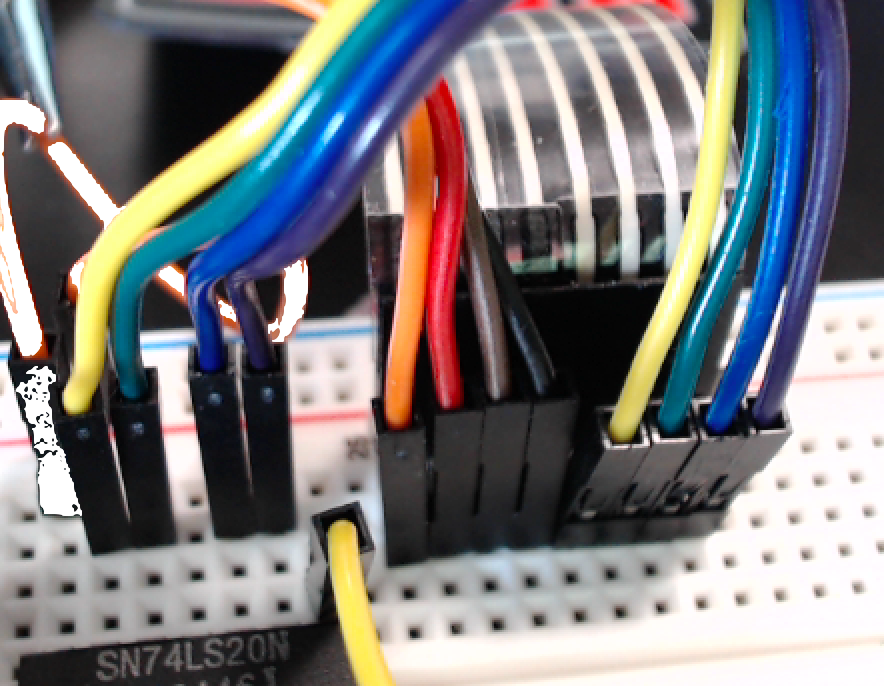
\includegraphics[width=.4\textwidth]{keypad/keypad-col-nand}
        \label{fig:keypad-col-nand}
    }
    \hfil
    \subfloat[Connection between the the 74LS20 and the \developmentboard's \texttt{A0}-\texttt{A3} pins.]{
        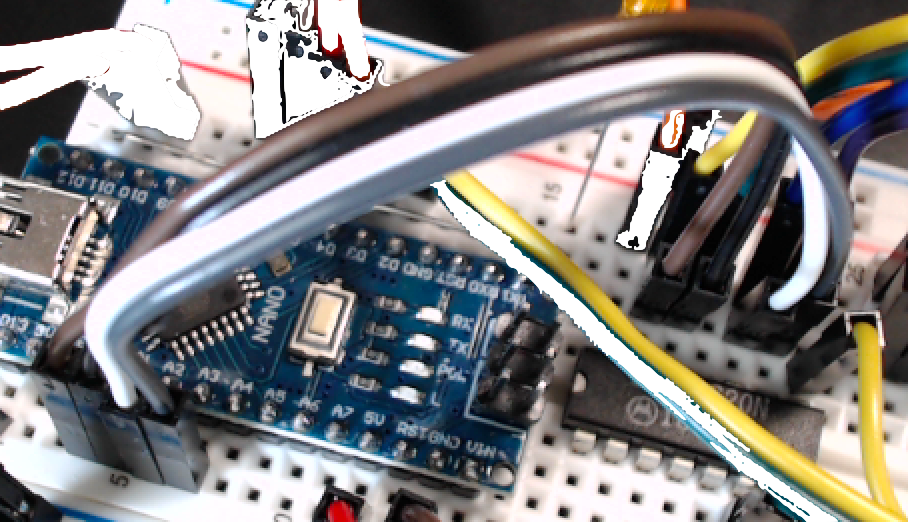
\includegraphics[width=.5\textwidth]{keypad/keypad-col-nano}
        \label{fig:keypad-col-nano}
    }
    \caption{Wiring the Matrix Keypad.}
\end{figure}

When you have finished setting up the keypad wiring, there should be the electrical paths described in Table~\ref{tab:keypad}.

\begin{table}
    \begin{center}\begin{tabular}{||c|c|c||} \hline\hline
    Keypad pin          & 74LS20            & \developmentboard\ pin \\ \hline
    \texttt{row1}       &                   & \texttt{D4} \\
    \texttt{row4}       &                   & \texttt{D5} \\
    \texttt{row7}       &                   & \texttt{D6} \\
    \texttt{row*}       &                   & \texttt{D7} \\
    \texttt{column1}    & Upper NAND Input  & \texttt{A0} \\
    \texttt{column2}    & Upper NAND Input  & \texttt{A1} \\
    \texttt{column3}    & Upper NAND Input  & \texttt{A2} \\
    \texttt{columnA}    & Upper NAND Input  & \texttt{A3} \\
                        & Upper NAND Output & \texttt{D3} \\ \hline\hline
    \end{tabular}\end{center}
    \caption{Electrical Paths for Matrix Keypad.\label{tab:keypad}}
\end{table}

\checkpoint{inserted and wired the matrix keypad}

In the Arduino IDE, open \textit{InputTest.ino}.
Connect your \developmentboard\ to the computer.
Compile \textit{InputTest.ino} and upload it to your \developmentboard.
Open the IDE's Serial Monitor (\textit{Tools} $\rightarrow$ \textit{Serial Monitor}).
You will see several lines reporting the current value of various inputs. (You will also see the \developmentboard's \texttt{TX} LED blinking as the \developmentboard\ sends these lines to your computer.)
Right now, KEYPAD~COLUMNS is always 1111, and KEYPAD~NAND is always 0.
Notice that when you press 1, 4, 7, or *, KEYPAD~COLUMNS becomes 0111;
similarly, pressing a button in the 2$^{nd}$ column causes KEYPAD~COLUMNS to become 1011;
in the 3$^{rd}$ column, 1101;
and in the A$^{th}$ column, 1110.
Whenever any keypad button is pressed, KEYPAD~NAND becomes 1.
Be sure to test all 16 keys.